% Section 2
% 2021-08-19
% Alessandro Zanatta

\section{Tools description}
\label{section:foundations}

In this section we are going to see a brief overview on the foundations of Tamarin prover, Verifpal  and Proverif - the three tools we are going to compare.


\subsection{Tamarin prover}
Let us start with Tamarin prover. For a more
in-depth description and further information, see the Tamarin foundations paper \cite{TamarinFoundations} or the extended foundations paper \cite{TamarinFoundationsExtended}.

The security property model of Tamarin is based on labelled multiset rewriting rules to specify protocols and adversary capabilities, a guarded fragment\footnote{The guarded fragment used by Tamarin is basically a subset of formulas from the first order logic with additional constraints on the arguments. See \cite{FragmentFirstOrderLogicPaper} for a definition from a mathematical point of view.} of first order logic to specify security properties and functions and equational theories to model the algebraic properties of cryptographic protocols \cite{TamarinFoundations}. Additionally, every event in the security properties is annotated with a timepoint $t \in \Q$ and basic comparison of timepoints can be used.

Tamarin then applies a constraint-solving algorithm based on backward-search and heuristics which tries to validate or falsify security properties.

\subsubsection{Multiset rewriting system}
The ingredients of Tamarin multiset rewriting system are the following:

\begin{itemize}
    \item{\textbf{Terms} - which can be thought of as messages;}
    \item{\textbf{Facts} - which model information in the protocol and are composed by terms;}
    \item{\textbf{State of the system} - which is represented using a \textit{multiset} of facts;}
    \item{\textbf{Transition rules} - which defines the possible transitions from one state to another. We will use the following syntax: $\msr{L}{A}{R}$, where $L$, $A$ and $R$ are multisets of facts, respectively called premises, actions and conclusions;}
    \item{\textbf{Trace} - a sequence $\left<A_1, \dots, A_n\right>$ of sets of ground facts (i.e. facts which do not contain any variable) denoting the sequence of \textit{actions} that happened during a protocol execution.}
\end{itemize}

\comment{
    \subsubsection{Constraint-solving procedure}
    \Cref{pseudocode:tamarin-solving-procedure} shows an high level view of the constraint-solving procedure of Tamarin. This solving procedure is based on a backward-search algorithm.

    \begin{algorithm}
        \begin{algorithmic}
            \Function{Solve}{\textphi}
            \EndFunction
        \end{algorithmic}
        \caption{Tamarin's constraint solving procedure}
        \label{pseudocode:tamarin-solving-procedure}
    \end{algorithm}
}

\subsection{Verifpal}

% TODO explain a bit of the syntax of verifpal!!!!

Verifpal also supports phases like Proverif (of course, with a different syntax).

\begin{figure}[t]
    \makebox[\textwidth][c]{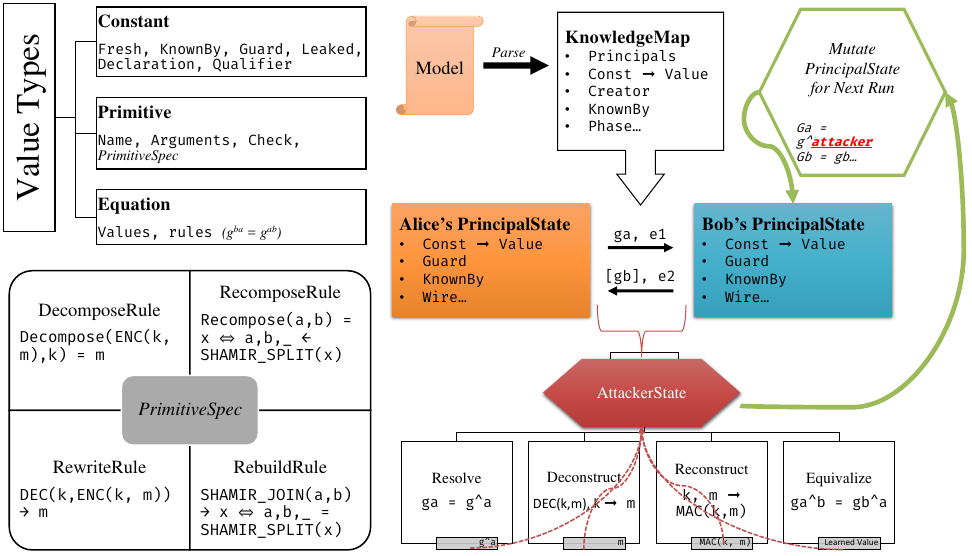
\includegraphics[scale=.6]{verifpal-internals}}
    \centering
    \caption{Verification process of Verifpal.\\ All credits to Nadim Kobeissi \cite{VerifpalManual}.}
    \label{fig:verifpal-verification}
\end{figure}

\Cref{fig:verifpal-verification} shows the process of protocol verification used by Verifpal. Let us describe the 5 main steps:

\begin{enumerate}
    \item{\textbf{Gather values} - first of all, the attacker passively observes a protocol execution and gathers all the values shared on the public channel between parties;}
    \item{\textbf{Populate attacker state} - gathered values are inserted into the attacker's state;}
    \item{\textbf{Apply transformations} - the attacker applies the four transformations on all of the obtained value (see bottom-right squares in \cref{fig:verifpal-verification});}
    \item{\textbf{Prepare next mutations} - if the attacker has learnt new values due to the transformations, it creates a combinatorial table of all possible substitutions and use it to derive a set of possible value substitutions across future executions of the protocol;}
    \item{\textbf{Mutate protocol executions} - finally, the attacker proceeds to execute the protocol, each time applying a mutation from the previous step. As long as the attacker keeps on learning new values, this entire process of gathering, populating, transforming, preparing and mutating is repeated.}
\end{enumerate}

Verifpal, after each stage, checks if any defined security property has been falsified (e.g. the attacker state contains a certain message).

\subsection{Proverif}


\begin{figure}[t]
    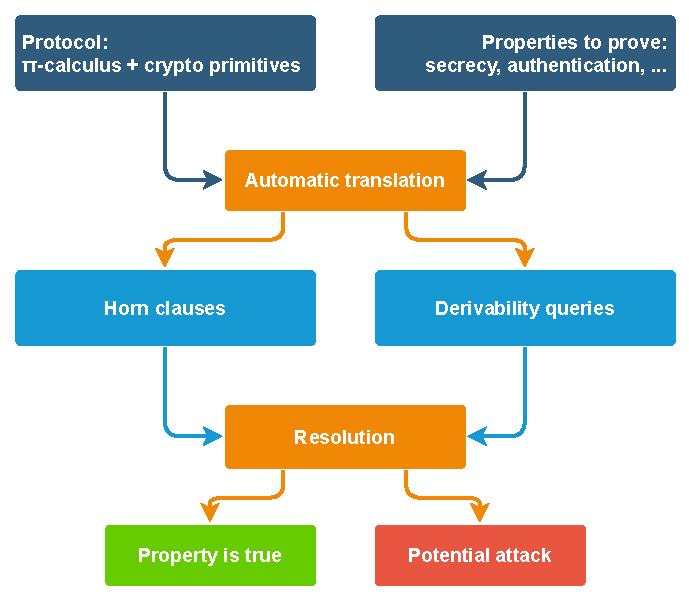
\includegraphics[scale=.8]{proverif-verification-method}
    \centering
    \caption{Proverif verification method.\\Inspired by a representation from Bruno Blanchet \cite{SymbolicComputationalBlanchet}.}
    \label{fig:proverif-verification-method}
\end{figure}

Proverif protocols and security properties are based on an extended version of the \pic (the \textit{applied} \picnospace). The tool also allows the user to define constructors, destructors and equations\footnote{Destructors are basically used to de-construct some previously constructed term (e.g. decryption of an encrypted ciphertext), while equations represent term equality of some sort (e.g. commutativity of multiplication).}, which form the cryptographic primitives. The protocol is then automatically translated to a set of Horn-clauses. Using this abstract representation of the protocol (based on Horn-clauses), the Proverif verifier uses a resolution algorithm on such clauses that allows for verification of security properties \cite{SymbolicComputationalBlanchet}.
A graphical representation of the whole process is given in \cref{fig:proverif-verification-method}.

A brief definition of the grammar of processes of the applied \pic is given in \cref{eq:apic-processes}. This syntax is identical to the one actually used by Proverif.

\lstset{language=proverif}
\begin{lstlisting}
0                  (* null process *)
out(N, M); P       (* output to channel N the message M *)
in(N, M: T); P     (* input from channel N of message M of sort T *)
P | Q              (* parallel composition *)
!P                 (* infinite replication *)
new a: T; P        (* fresh value of sort T *)
if M then P else Q (* conditional*)
\end{lstlisting}

\lstset{language=proverif}
The null process \lstinline{0} does nothing;
\lstinline{out(N, M); P} (\lstinline{in(N, M: T); P}) outputs (gets) the message \lstinline{M} (of sort \lstinline{T}) into (from) channel \lstinline{N} and then continues with process \lstinline{P};
\lstinline{P | Q} is the parallel composition of \lstinline{P} and \lstinline{Q};
The process \lstinline{!P} effectively behaves as an infinite number of copies of \lstinline{P} running in parallel (\textit{unbounded} replication);
\lstinline{new a: T; P} creates a new fresh value of sort \lstinline{T}, before proceeding with process \lstinline{P};
\lstinline{if M then P else Q} if a standard conditional.

\lstset{language=proverif}
There are many additions to this grammar, such as:
\begin{itemize}
    \item{\lstinline{event EventName(x, y);} - allows to define a trace of events on which security properties can be defined;}
    \item{\lstinline{query event(EventName(x, y))} - queries are used to define security properties. The reserved word \lstinline{attacker(x)} allows to ask Proverif if the attacker knows the term $x$;}
    \item{\lstinline{phase t;} - allows to execute a process only after processes of phases $< t$ have been executed. Intuitively, $t$ can be thought of as a global clock and a process in phase $t$ is active only during phase $t$.}
\end{itemize}